\begin{atiTask}[
  title = Anwendbarkeit des GAUSSschen Satzes %Klammern werden benötigt für die Kapitälchen
  %call = Zusatzaufgabe,
]

Gegeben sei das Vektorfeld
\[
\vec{F}=\frac{\vec{r}}{r^3},\quad r=\sqrt{x^2+y^2+z^2}.
\]
\begin{atiSubtasks}
\item Berechen Sie die Divergenz dieses Vektorfeldes.
\item Berechnen Sie den Fluss
\[\oiint\limits_{S_1} \vec{F}\;\mathrm{d}\vec{f},
\]
worin $S_1$ die Einheitskugel mit ihrem Mittelpunkt im Korrdiantenursprung sein soll, direkt aus dem Oberflächenintegral. Kann man dieses Integral mit Hilfe des \textsc{Gauss}schen Satzes berechnen? Begründen Sie kurz!
\item Wiederholen Sie die Berechnung des Flusses für eine Fläche $S_2$, die die Einheitskugel ist, deren Mittelpunkt der Punkt $M(0,0,2)$ liegt. Verifizieren Sie das Resultat mit Hilfe des \textsc{Gauss}schen Satzes, falls dieser anwendbar ist. 
\end{atiSubtasks}
\atiNote{für das Oberflächenintegral: Verschieben Sie den Ursprung des Koordinatensystems in den Punkt $M$.}

\end{atiTask}

\begin{atiSolution}
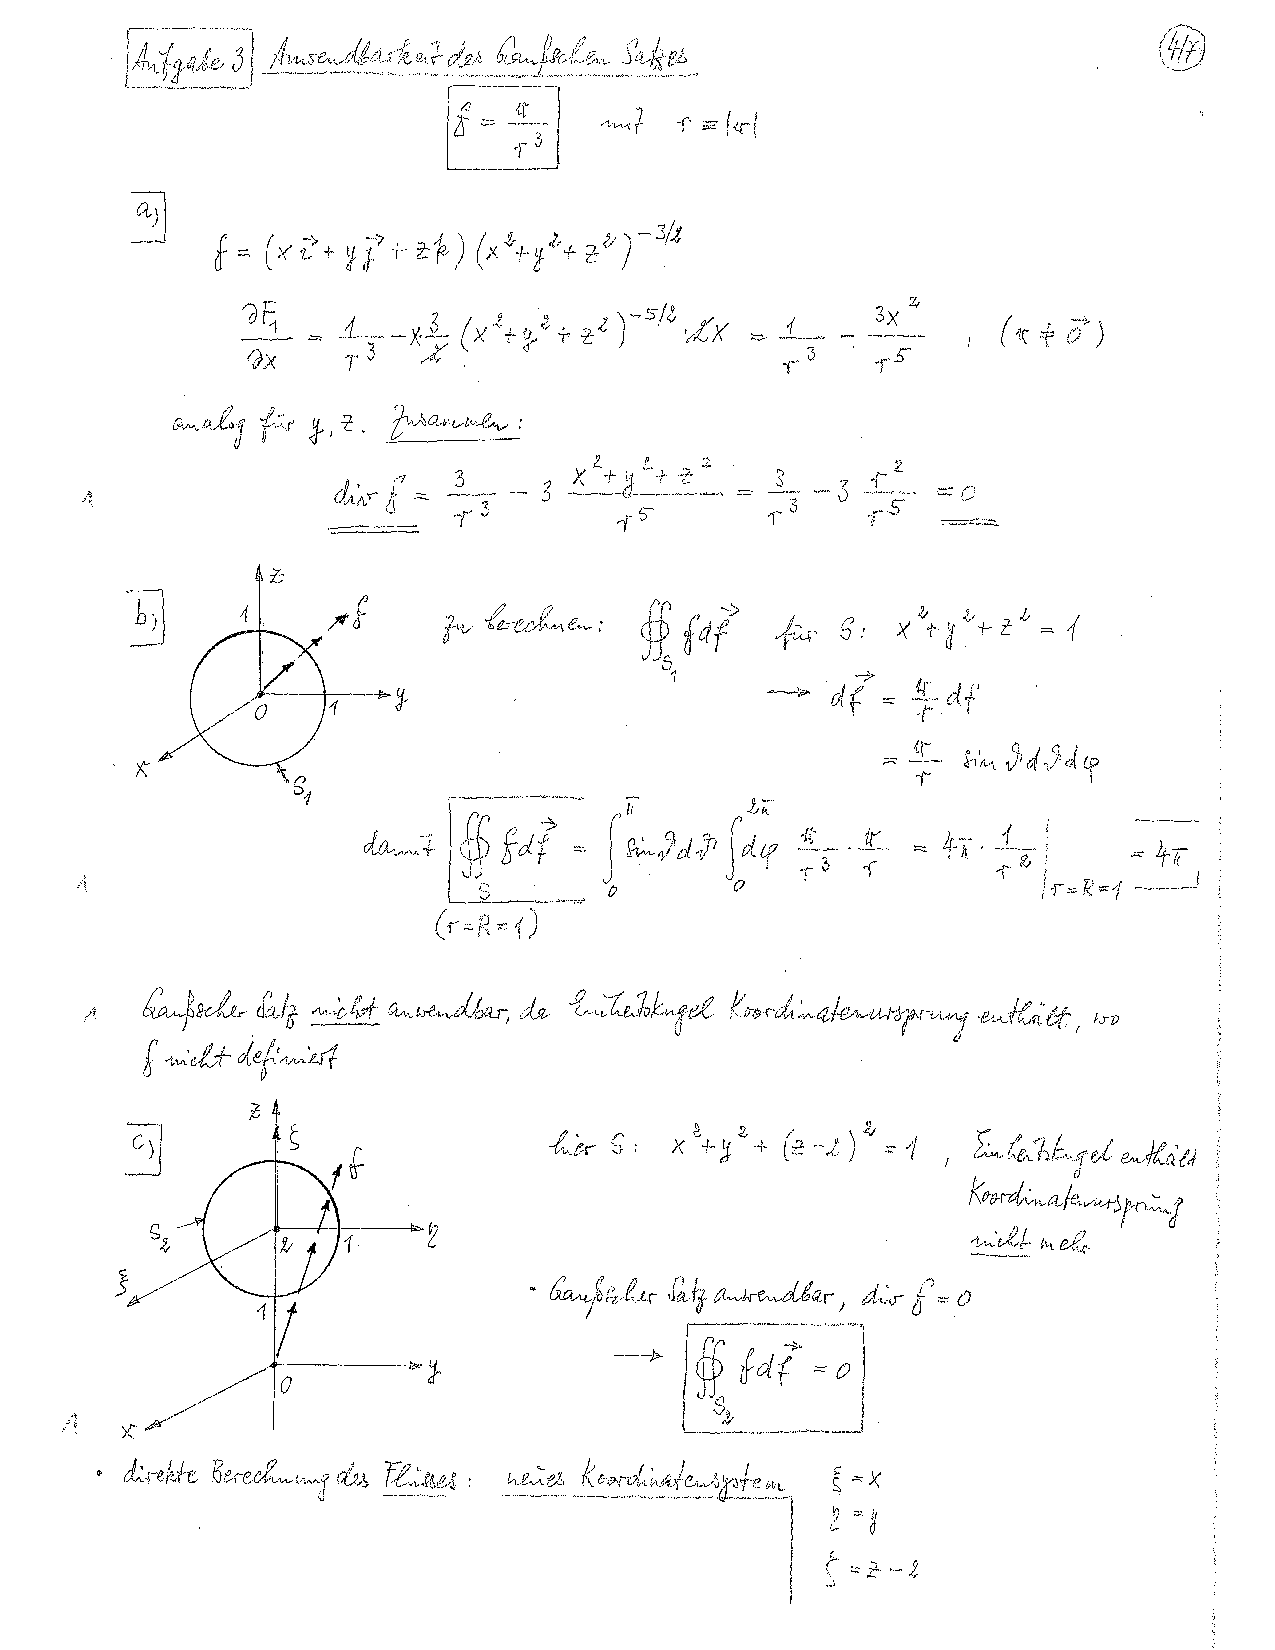
\includepdf[pages=-]{solution-gauss_ii.pdf}
\end{atiSolution}